%%===========================================================%%
%%                                                           %%
%%   FORMULATION OF TOTAL RP EFFICIENCY CORRECTION APPENDIX  %%
%%                                                           %%
%%===========================================================%%

\chapter{Reconstruction of \texorpdfstring{$\bf{m}^{2}_{\text{\small TOF}}$}{mTOF^2}}\label{appendix:squaredMass}


\textbf{Definitions:}\\[7pt]
\begin{tabular}{ll}
$t_{0}$ &- time of the primary $pp$ interaction\\
$t_{1,2}$ &- time of detection of the hit in TOF by particle 1(2)\\
$L_{1,2}$ & - helical path of the particle 1(2) from the interaction vertex to the TOF cell with reconstructed hit,\\
$p_{1,2}$ & - magnitude of momentum of particle 1(2),\\
$m_{1,2}$ & - mass of particle 1(2),\\
\end{tabular}\vspace{10pt}


%---------------------------
\begin{figure}[ht!]
\centering%
\parbox{0.29\textwidth}{%
  \centering%
  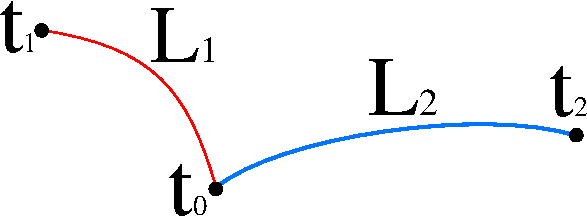
\includegraphics[width=\linewidth]{graphics/eventSelection/TofScheme.pdf}\label{fig:tofScheme}
}%
\quad\quad%
\parbox{0.655\textwidth}{%
    \caption[Scheme of two central tracks with common vertex, hitting cells in TOF detector.]{Scheme of two central tracks of lengths $L_{1}$ and $L_{2}$, produced in common vertex in moment $t_{0}$, hitting cells in TOF detector in moments $t_{1}$ and $t_{2}$.}
}%

\end{figure}
%---------------------------


From the simple algebra below which describes relation between track lengths, momenta and times of hit detection one can derive formula for the squared mass of two particles, assuming that their masses are equal (particles are of the same type).

Below we assume $c=1$. We can write a set of two equations connecting the time that it takes for each particle to reach the TOF, starting from the interaction vertex:
\begin{equation}
 \left\{\begin{array}{l}%
 t_{1}-t_{0} = L_{1}\sqrt{1+\frac{m_{1}^{2}}{p_{1}^{2}}}, \\[3pt]
 t_{2}-t_{0} = L_{2}\sqrt{1+\frac{m_{2}^{2}}{p_{2}^{2}}}.
\end{array}\right.%
\end{equation}
By adding the two equations above we get
\begin{equation}\label{eq:m2Temp}
 \Delta t = t_{1}-t_{2} = L_{1}\sqrt{1+\frac{m_{1}^{2}}{p_{1}^{2}}} - L_{2}\sqrt{1+\frac{m_{2}^{2}}{p_{2}^{2}}}.
\end{equation}
In CEP of two opposite-sign particles always the same species of particles are produced, therefore
\begin{equation}m_{1}=m_{2}=m.\end{equation}
If we substitute $m_{1}$ and $m_{2}$ with $m$ in Eq.~\eqref{eq:m2Temp} and transform the equation to remove the square roots we get a quadratic equation of the form 
\begin{equation}\label{eq:m2Quad}\mathcal{A}\times \left(m^{2}_{\text{\tiny TOF}}\right)^{2} + \mathcal{B}\times m^{2}_{\text{\tiny TOF}} + \mathcal{C} = 0.\end{equation}
Parameters of the Eq.~\eqref{eq:m2Quad} are given below:
\begin{equation}
\mathcal{A}= -2\frac{L^2_1L^2_2}{p^2_1p^2_2}+\frac{L^4_1}{p^4_1}+\frac{L^4_2}{p^4_2},
\end{equation}
\begin{equation}
\mathcal{B}=-2L^2_1L^2_2\left({\frac{1}{p^2_1}} + {\frac{1}{p^2_2}}\right)+\frac{2L^4_1}{p_1^2}+\frac{2L^4_2}{p_2^2}-2\left(\Delta t\right)^2\left(\frac{L^2_1}{p_1^2}+\frac{L^2_2}{p_2^2}\right),
\end{equation}
\begin{equation}
\mathcal{C}=\left(\Delta t\right)^4-2\left(\Delta t\right)^2\left(L^2_1+L^2_2\right)+L^4_1+L^4_2-2L^2_1L^2_2,
\end{equation}
together with the final formula for a physical root of the quadratic equation which is used in the $m^{2}_{\text{\tiny TOF}}$ reconstruction:
\begin{equation}
 \label{eq:mSquared}
m^{2}_{\text{\tiny TOF}} = \frac{-\mathcal{B}+\sqrt{\mathcal{B}^2-4\mathcal{A}\mathcal{C}}}{2\mathcal{A}}.
\end{equation}
